\chapter{Visual--inertial odometry}
\label{ch:vio}

The camera and the IMU fail in opposite ways. The camera sees the world
and does not drift while it sees the same landmarks, but it is blind in
a uniform hedge, against the sun, or when the image blurs in a fast
turn. The IMU sees nothing, but it never stops measuring, two hundred
times per second; its integration drifts within seconds
(\cref{prop:drift}), but over the fraction of a second between two
keyframes it is excellent. Fused, they give \emph{visual--inertial
odometry} (VIO), which is more accurate than either and survives short
blind spells. Gravity also enters the problem: the IMU makes roll and
pitch observable, and leaves only four directions in which the estimate
can drift.

This chapter builds a sliding-window VIO from the pieces of the previous
chapters: the stereo reprojection factor of Chapter~\ref{ch:ba}, the IMU
factor of Chapter~\ref{ch:imu}, and the marginalisation of
Chapter~\ref{ch:posegraph}. It then studies what the fused system can and
cannot observe, how to start it, what the filtering alternative (the
MSCKF) does instead, and what an uncalibrated time offset between the
two sensors costs.

\section{Filtering or smoothing}

Visual--inertial estimators come in two families. \emph{Filters} keep a
state and its covariance and update them with each measurement. The
most successful is the multi-state constraint Kalman filter (MSCKF) of
Mourikis and Roumeliotis, whose open-source descendant OpenVINS is a
reference implementation. \emph{Smoothers} keep a window of recent
keyframe states, optimise all of them with all the measurements that
link them, and marginalise the oldest keyframe when the window is full.
OKVIS, VINS-Mono and ORB-SLAM3 are of this kind. Chapter~\ref{ch:slam}
explained why smoothing is the default today: it relinearises, so it is
more accurate when the problem is nonlinear. Filters are cheaper and
remain the choice on very small processors. This chapter implements the
smoother and explains the key step of the filter.

\section{The visual factor with an inertial state}

The VIO state of keyframe $k$ is $\vect{x}_k=(R_k,\vect{v}_k,\p_k,
\vect{b}_{g,k},\vect{b}_{a,k})$, 15 degrees of freedom: the pose of the
\emph{body} (IMU) frame, its velocity and the two biases, perturbed as in
Chapter~\ref{ch:imu}. The camera is attached to the body by the
extrinsic transformation $T_{BC}=(R_{BC},\vect{t}_{BC})$, so the camera
pose is $R_c=R_kR_{BC}$, $\vect{c}=\p_k+R_k\vect{t}_{BC}$, and a world
point $\vect{X}$ has camera coordinates $\vect{q}=R_c\T(\vect{X}-\vect{c})$.
The stereo projection of $\vect{q}$ is the one of \cref{def:ba}.

\begin{proposition}{Jacobians of the camera point}{viojac}
With $R_k\leftarrow R_k\Exp(\delta\bphi)$, $\p_k\leftarrow\p_k+R_k\,
\delta\p$ and $\vect{X}\leftarrow\vect{X}+\delta\vect{X}$, to first order
\begin{equation}\label{eq:viojac}
\frac{\partial\vect{q}}{\partial\delta\bphi}=\hatop{\vect{q}}\,R_{BC}\T+
R_{BC}\T\hatop{\vect{t}_{BC}},\qquad
\frac{\partial\vect{q}}{\partial\delta\p}=-R_{BC}\T,\qquad
\frac{\partial\vect{q}}{\partial\delta\vect{X}}=R_c\T,
\end{equation}
and $\vect{q}$ does not depend on $\vect{v}_k$ or the biases.
\end{proposition}

\begin{proof}
Perturbing the rotation and the position,
$R_k\Exp(\delta\bphi)R_{BC}=R_c\Exp(R_{BC}\T\delta\bphi)$ by
\eqref{eq:so3id}, and $\vect{c}$ becomes
$\p_k+R_k\delta\p+R_k\Exp(\delta\bphi)\vect{t}_{BC}\approx\vect{c}+R_k
\delta\p-R_k\hatop{\vect{t}_{BC}}\delta\bphi$. Hence
\[
\vect{q}'\approx\bigl(I-\hatop{(R_{BC}\T\delta\bphi)}\bigr)R_c\T
\bigl(\vect{X}-\vect{c}-R_k\delta\p+R_k\hatop{\vect{t}_{BC}}\delta\bphi
\bigr).
\]
Expanding to first order with $R_c\T R_k=R_{BC}\T$ and
$-\hatop{\vect{a}}\vect{q}=\hatop{\vect{q}}\vect{a}$ gives
$\vect{q}'\approx\vect{q}+\hatop{\vect{q}}R_{BC}\T\delta\bphi-R_{BC}\T
\delta\p+R_{BC}\T\hatop{\vect{t}_{BC}}\delta\bphi$. The point enters
linearly through $R_c\T\vect{X}$.
\end{proof}

The residual Jacobians are those of $\vect{q}$ multiplied by the
projection Jacobian (\cref{prop:projjac}), as in Chapter~\ref{ch:ba}.

\section{The sliding window}

\begin{definition}{Sliding-window VIO}{swvio}
Let the window hold keyframes $k=1,\dots,N$ and landmarks $\vect{X}_l$.
The estimate minimises
\begin{equation}\label{eq:swcost}
F=\tfrac12\sum_{(k,l)}\rho\bigl(\norm{\vect{r}_{kl}}^2\bigr)
+\tfrac12\sum_{k=1}^{N-1}\Bigl(\norm{\vect{r}^{\mathrm{imu}}_{k,k+1}}^2_{
\Sigma_{k,k+1}^{-1}}+\norm{\vect{b}_{k+1}-\vect{b}_k}^2_{\Sigma_b^{-1}}
\Bigr)+F_{\mathrm{prior}}(\vect{x}_{1:N}),
\end{equation}
where $\vect{r}_{kl}$ is the whitened stereo residual of landmark $l$ in
keyframe $k$, $\rho$ is the Huber kernel, $\vect{r}^{\mathrm{imu}}$ is the
IMU factor (\cref{def:imufactor}), $\Sigma_b$ the bias random walk over
the interval, and $F_{\mathrm{prior}}$ a quadratic prior on the states,
from the initialisation and then from marginalisation.
\end{definition}

The implementation, \code{vio.SlidingWindowVIO}, keeps $N=8$ keyframes
taken at 4\,Hz (every fifth frame of a 20\,Hz stereo camera), 2\,s of
motion. With every new keyframe it:
\begin{enumerate}[nosep]
\item preintegrates the IMU samples since the previous keyframe, at the
  previous keyframe's bias estimate, and predicts the new state
  (\cref{thm:preint});
\item triangulates the new landmarks from the stereo pair at the
  predicted pose, at most 120 per keyframe;
\item runs a few Levenberg--Marquardt iterations on \eqref{eq:swcost},
  eliminating the landmarks with the Schur complement exactly as in
  \cref{thm:schurba}. The reduced system has $15N=120$ unknowns, against
  some 670 landmarks;
\item removes the observations whose whitened error exceeds the 99\,\%
  point of $\chi^2_3$;
\item if the window holds more than $N$ keyframes, marginalises the
  oldest one.
\end{enumerate}

Marginalisation follows \cref{prop:margprior}. The oldest keyframe is
removed together with every landmark it observes and \emph{all} the
observations of those landmarks, also those made from the other
keyframes in the window. The factors removed (the old prior, the first
IMU and bias factors, and those observations) are linearised at the
current estimate, and both the keyframe and the landmarks are eliminated
by the Schur complement (\cref{lem:schur}). What remains is a dense
Gaussian prior on the remaining states only. Removing the landmarks
with all their observations is what keeps the prior free of
landmarks, so that the reduced system keeps its structure. Each
observation enters the prior once and leaves the window at the same
time, so nothing is counted twice. A track that continues to be
observed simply becomes a new landmark. This is, in substance, the
strategy of VINS-Mono.

The prior is linearised once and never again: as the states it involves
move, its Jacobians stay those of the old linearisation point, while the
factors added later are linearised at the new estimate. This is the
inconsistency of \cref{prop:fej}, and \emph{first-estimate Jacobians}
are its standard fix; our implementation does without, and pays for it
with slightly overconfident estimates.

\section{What the fusion can observe}

A visual--only system is blind to a rigid motion of the whole map and
trajectory: six gauge directions (\cref{prop:gauge}). The IMU adds
gravity, a vector known in the world frame, which fixes two of the
three rotations.

\begin{theorem}{Four unobservable directions}{vionull}
Let $Q=\Exp(\theta\vect{e}_z)$ be a rotation about the direction of
gravity and $\vect{t}\in\R^3$. The transformation
\[
R_k\mapsto QR_k,\quad\vect{v}_k\mapsto Q\vect{v}_k,\quad\p_k\mapsto Q\p_k+
\vect{t},\quad\vect{X}_l\mapsto Q\vect{X}_l+\vect{t},\quad\vect{b}_k
\mapsto\vect{b}_k
\]
leaves every residual of \eqref{eq:swcost} without prior unchanged. In
the local coordinates of the window, the four directions
\begin{equation}\label{eq:vionull}
\begin{aligned}
\text{translation }\vect{t}:&\quad\delta\p_k=R_k\T\vect{t},\quad
\delta\vect{X}_l=\vect{t},\\
\text{yaw}:&\quad\delta\bphi_k=R_k\T\vect{e}_z,\quad\delta\vect{v}_k=
\vect{e}_z\times\vect{v}_k,\quad\delta\p_k=R_k\T(\vect{e}_z\times\p_k),\quad
\delta\vect{X}_l=\vect{e}_z\times\vect{X}_l,
\end{aligned}
\end{equation}
with all other components zero, are in the null space of the Jacobian of
the residuals, hence of the Gauss--Newton Hessian, at every estimate.
\end{theorem}

\begin{proof}
\emph{Visual residuals.} The camera pose becomes $(QR_c,Q\vect{c}+
\vect{t})$, so $\vect{q}=(QR_c)\T(Q\vect{X}+\vect{t}-Q\vect{c}-\vect{t})=
R_c\T(\vect{X}-\vect{c})$ is unchanged.

\emph{IMU residuals.} $(QR_i)\T QR_j=R_i\T R_j$, so the rotation residual
is unchanged. For the velocity, $(QR_i)\T(Q\vect{v}_j-Q\vect{v}_i-\vect{g}
\Delta t)=R_i\T(\vect{v}_j-\vect{v}_i-Q\T\vect{g}\Delta t)$, and $Q\T
\vect{g}=\vect{g}$ because $Q$ rotates about $\vect{g}$. The position
residual is the same, the translation $\vect{t}$ cancelling in $\p_j-
\p_i$. The biases do not move, so the bias factors and the bias
corrections are unchanged.

\emph{Directions.} Differentiate the transformation at $\theta=0$,
$\vect{t}=\vect{0}$ in local coordinates: $QR_k=R_k\Exp(R_k\T\vect{e}_z
\theta)$ gives $\delta\bphi_k$; $Q\p_k+\vect{t}=\p_k+R_k\delta\p_k$
gives $\delta\p_k=R_k\T(\theta\,\vect{e}_z\times\p_k+\vect{t})$; the
others are direct. Since the residual vector $\vect{r}$ is constant
along these curves, $J\vect{u}=\vect{0}$ for each direction $\vect{u}$,
so $J\T WJ\vect{u}=\vect{0}$ for any weights $W$.
\end{proof}

The theorem shows that at least four directions are unobservable.
Under general motion there are no others: roll and pitch are
observable, and so are velocities and biases (Jones and Soatto, Kelly
and Sukhatme, Hesch et~al.). Two kinds of motion that a ground vehicle
performs all the time are not general, though.

\begin{proposition}{Tilt and accelerometer bias without rotation}{tiltbias}
Suppose all keyframes of the window have the same rotation $R$. Let
$\delta\btheta\perp\vect{g}$ be a small horizontal rotation vector. Rotating
all states and landmarks by $\Exp(\delta\btheta)$ about the origin, and
changing every accelerometer bias by $\delta\vect{b}_a=-R\T(\delta\btheta
\times\vect{g})$, leaves the residuals of \eqref{eq:swcost} unchanged to
first order. With rotations about the vertical only, this no longer
holds.
\end{proposition}

\begin{proof}
The visual residuals are invariant under any rigid motion, as in the
proof of \cref{thm:vionull}. For the IMU, the specific force predicted
by the states is $R\T(\vect{a}-\vect{g})+\vect{b}_a$. After the
rotation it is $R\T\Exp(-\delta\btheta)(\Exp(\delta\btheta)\vect{a}-\vect{g})+
\vect{b}_a+\delta\vect{b}_a=R\T(\vect{a}-\vect{g})+R\T(\delta\btheta\times
\vect{g})+\vect{b}_a+\delta\vect{b}_a$ to first order, using
$\Exp(-\delta\btheta)\vect{g}\approx\vect{g}-\delta\btheta\times\vect{g}$. The
choice of $\delta\vect{b}_a$ cancels the change, at every instant,
because $R$ is constant. So the preintegrated measurements and the
predicted ones change together, and the bias factors see a constant
shift. If $R$ varies by rotations $R_z(\psi)$ about the vertical,
$R_z(\psi)\T(\delta\btheta\times\vect{g})$ varies with $\psi$ (the vector
$\delta\btheta\times\vect{g}$ is horizontal), and no constant bias change
compensates it.
\end{proof}

\begin{inwords}
On a straight row, a slightly tilted estimate with a slightly wrong
accelerometer bias explains the data as well as the truth: gravity seen
through a tilt of $\delta\theta$ looks like a bias of $g\,\delta\theta$
(Exercise~\ref{ex:12tilt}). Only rotation separates them: in a turn the
bias rotates with the body, while the tilt error does not. A mower turns
at the end of every row, and that is when its accelerometer bias
becomes known.
\end{inwords}

\begin{figure}[ht]
\centering
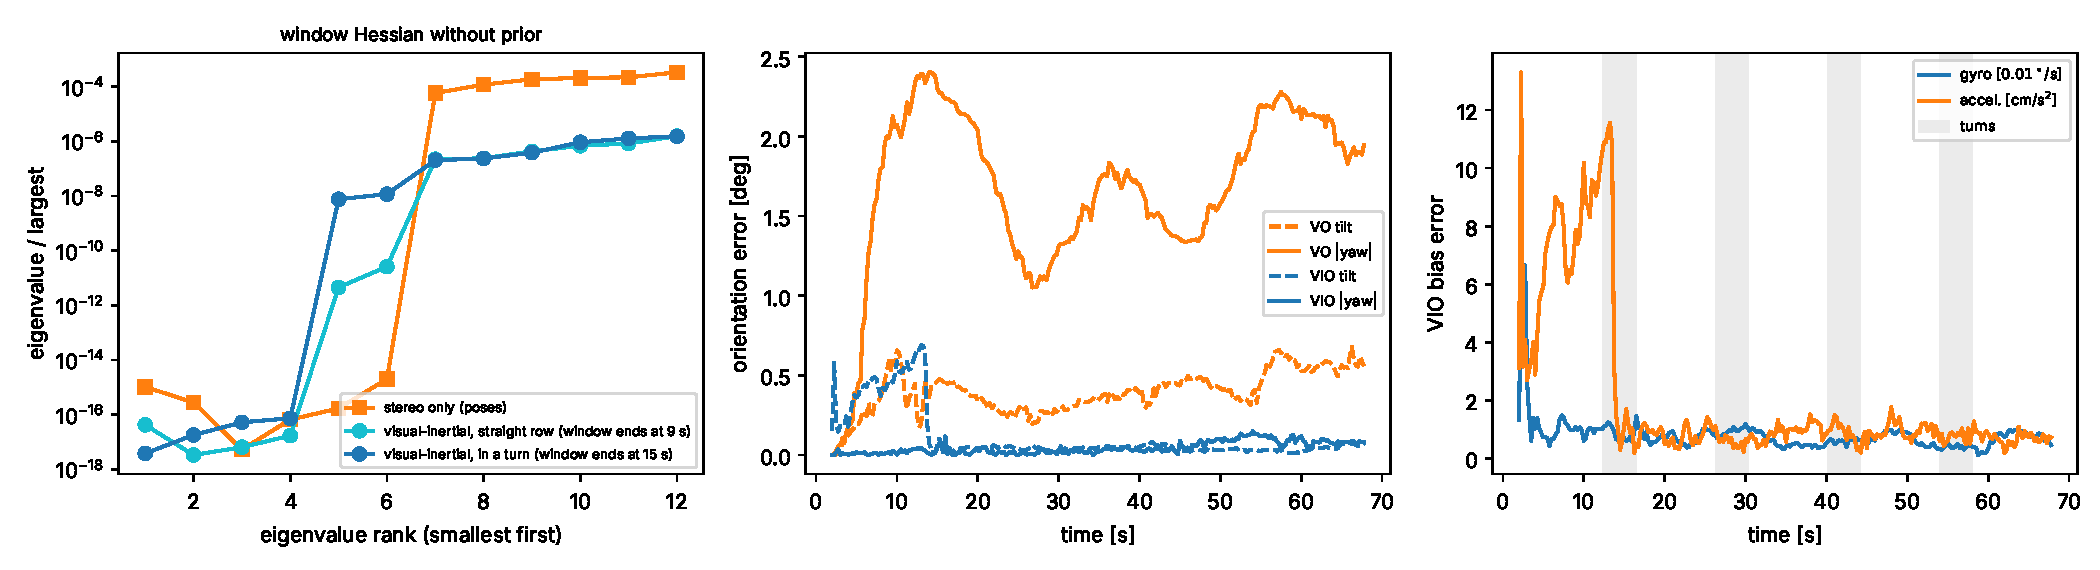
\includegraphics[width=\linewidth]{figures/ch13_obs.pdf}
\caption{Left: smallest eigenvalues of the Gauss--Newton Hessian of a
window (landmarks eliminated, no prior). Stereo only (poses): six zero
eigenvalues. Visual--inertial: four zero eigenvalues (\cref{thm:vionull})
and, on a straight row, two more that are tiny (\cref{prop:tiltbias});
they grow by four orders of magnitude when the window contains a turn.
Middle: tilt and yaw errors of the stereo VO and of the VIO along the
drive. Right: bias errors of the VIO; grey bands are the turns.}
\label{fig:vioobs}
\end{figure}

\Cref{fig:vioobs} checks both statements on the garden drive.
\begin{itemize}[nosep]
\item The Hessian of a window has exactly four zero eigenvalues (to
  $10^{-17}$ of the largest), and the test suite checks that they are the
  directions \eqref{eq:vionull}.
\item On a straight row, two more eigenvalues are tiny ($10^{-12}$ and
  $10^{-11}$): the small pitch and roll of the bumpy lawn are all that
  separate tilt from bias.
\item The accelerometer bias error of the VIO is about 0.1\,m/s$^2$
  until the first turn, and drops below 0.01\,m/s$^2$ during it.
\item The tilt error, up to $0.7^\circ$ before the turn (the static
  initialisation's error, $|\vect{b}_a|/g$), falls to below $0.1^\circ$
  and stays there: gravity makes it observable. The yaw error does not
  grow much here, but nothing would bring it back if it did.
\item The stereo VO, without gravity, ends with a $0.6^\circ$ tilt error
  and a $2^\circ$ yaw error.
\end{itemize}

\section{The filter's trick: the MSCKF}

A filter cannot keep the landmarks in its state: there are too many.
The MSCKF keeps the IMU state and a sliding window of past camera poses,
and uses a feature only when its track ends. It then triangulates the
feature from the window poses, linearises the reprojection errors of
its $m$ observations as
\begin{equation}\label{eq:msckflin}
\vect{r}=H_x\,\delta\vect{x}+H_f\,\delta\vect{f}+\vect{n},\qquad
\vect{n}\sim\Normal(0,\sigma^2I_{m}),
\end{equation}
with $H_f$ of size $m\times3$ and full column rank, and removes the
feature by projecting onto the left null space of $H_f$.

\begin{proposition}{Null-space projection marginalises the feature}{msckf}
Let the columns of $N$ ($m\times(m-3)$) be an orthonormal basis of the
left null space of $H_f$, $N\T H_f=0$. The projected measurement
$\vect{r}_o=N\T\vect{r}=N\T H_x\delta\vect{x}+N\T\vect{n}$ does not involve
$\delta\vect{f}$, has white noise $N\T\vect{n}\sim\Normal(0,\sigma^2
I_{m-3})$, and carries exactly the information on $\delta\vect{x}$ that
remains after marginalising $\delta\vect{f}$ out of \eqref{eq:msckflin}:
\begin{equation}\label{eq:msckfeq}
H_x\T NN\T H_x=H_x\T H_x-H_x\T H_f(H_f\T H_f)^{-1}H_f\T H_x,
\end{equation}
and likewise for the information vectors $H_x\T NN\T\vect{r}$.
\end{proposition}

\begin{proof}
$N\T H_f=0$ removes $\delta\vect{f}$, and $\mathrm{Cov}(N\T\vect{n})=
\sigma^2N\T N=\sigma^2I$. Let $P_f=H_f(H_f\T H_f)^{-1}H_f\T$ be the
orthogonal projector onto the range of $H_f$. The columns of $N$ span
the orthogonal complement of that range, so $NN\T=I-P_f$. Then
$H_x\T NN\T H_x=H_x\T H_x-H_x\T P_fH_x$, which is the right-hand side of
\eqref{eq:msckfeq}. That is the Schur complement of the $\delta
\vect{f}$ block in the information matrix of \eqref{eq:msckflin}
(\cref{lem:schur}); the information vectors follow in the same way.
\end{proof}

So the MSCKF and the smoother do the same thing with a feature, at the
first order: marginalise it. The filter does it once per feature, with
the Jacobians of that moment, and the update is then final; the smoother
keeps the landmark while it is in the window and may relinearise it.
The filter's cost is linear in the number of features, and its update is
an EKF update with the stacked $\vect{r}_o$ (usually compressed first by
a QR decomposition). Consistency matters as much as for the smoother:
the observability-constrained and first-estimate-Jacobian variants of
the MSCKF (Huang et~al.; Li and Mourikis) exist because the naive filter
gains spurious information about yaw.

\section{Starting up}

The window needs a first state: rotation, velocity, biases. Position and
yaw are the gauge and can be set freely; the rest must be estimated.

\begin{proposition}{Static initialisation}{staticinit}
If the IMU is at rest over $n$ samples, the mean gyroscope reading
estimates $\vect{b}_g$, with standard deviation $\sigma_g/\sqrt{T}$ per
axis over a duration $T$. The mean accelerometer reading $\bar{\vect{f}}=
R\T(-\vect{g})+\vect{b}_a+\text{noise}$ determines the vertical in the
body frame, $R\T\vect{e}_z\approx\bar{\vect{f}}/\norm{\bar{\vect{f}}}$,
hence roll and pitch, with an error of about $|\vect{b}_a^\perp|/g$,
where $\vect{b}_a^\perp$ is the horizontal part of the bias. Yaw is not
determined.
\end{proposition}

\begin{proof}
At rest $\bomega=\vect{0}$ and $\vect{a}=\vect{0}$, so the samples are
$\vect{b}_g+\vect\eta_g$ and $R\T(-\vect{g})+\vect{b}_a+\vect\eta_a$. The
mean of $n$ white samples of standard deviation $\sigma_g/\sqrt{\Delta t}$
has standard deviation $\sigma_g/\sqrt{n\Delta t}$. For the
accelerometer, $-R\T\vect{g}=g\,R\T\vect{e}_z$, and a bias component
perpendicular to it tilts the measured vertical by $\arctan(|\vect{b}_a^
\perp|/g)$, as in Exercise~\ref{ex:12tilt}; yaw does not change $R\T
\vect{e}_z$.
\end{proof}

A mower starts at rest, so this is how our VIO starts: 2\,s in the shed
give the gyroscope bias to $0.01^\circ$/s and the tilt to the
accelerometer bias, here $0.7^\circ$. The first turn then corrects both
tilt and bias (\cref{fig:vioobs}). A system that starts in motion (a
drone thrown in the air, a car) needs \emph{dynamic} initialisation:
run vision alone for a second or two, then align the IMU to it.

\begin{proposition}{Visual--inertial alignment}{align}
Let keyframe poses $(R_k,\p_k)$ be known in some frame (from stereo VO),
and let $\Delta R_{k,k+1}$, $\Delta\vect{v}_{k,k+1}$, $\Delta\p_{k,k+1}$
be preintegrated between them.
\begin{enumerate}[nosep]
\item The gyroscope bias correction $\delta\vect{b}_g$ minimising
  \[
  \sum_k\norm{\Log\bigl((\Delta R_{k,k+1}\Exp(J^R\delta\vect{b}_g))\T
  R_k\T R_{k+1}\bigr)}^2
  \]
  is, to first order, the linear least-squares solution of the equations
  $J^R_{k,k+1}\delta\vect{b}_g=\Log(\Delta R_{k,k+1}\T R_k\T R_{k+1})$,
  $k=1,\dots,n-1$.
\item Given the bias, gravity $\vect{g}$ in that frame and the velocities
  $\vect{v}_k$ solve the linear system
  \begin{equation}\label{eq:align}
  \vect{v}_{k+1}-\vect{v}_k-\vect{g}\Delta t_k=R_k\Delta\vect{v}_{k,k+1},
  \qquad
  -\vect{v}_k\Delta t_k-\tfrac12\vect{g}\Delta t_k^2=R_k\Delta
  \p_{k,k+1}-(\p_{k+1}-\p_k).
  \end{equation}
\end{enumerate}
For a monocular camera the positions are known up to a scale $s$;
replacing $\p_k$ by $s\,\p_k$ keeps \eqref{eq:align} linear in
$(\vect{v}_k,\vect{g},s)$.
\end{proposition}

\begin{proof}
1. With the bias Jacobian, $\Delta R(\vect{b}_g+\delta\vect{b}_g)\approx
\Delta R\Exp(J^R\delta\vect{b}_g)$ (\cref{prop:preintbias}); the residual
is $\Log(\Exp(-J^R\delta\vect{b}_g)\Delta R\T R_k\T R_{k+1})\approx
\Log(\Delta R\T R_k\T R_{k+1})-J^R\delta\vect{b}_g$ to first order (the
Jacobian $J_r^{-1}$ of the logarithm is close to $I$ for the small
residual). Its sum of squares is minimised by the least-squares
solution. 2. These are the velocity and position relations of
\cref{thm:preint}, rearranged with the unknowns on the left.
\end{proof}

On the garden drive, aligning 2\,s of stereo VO started from an
arbitrary frame gives the direction of gravity to $0.23^\circ$ and its
magnitude as 9.833\,m/s$^2$; the gyroscope bias, $0.19^\circ$/s, is
recovered to $0.05^\circ$/s. ORB-SLAM3 refines such an estimate with a
small inertial-only optimisation before starting the full VIO.

\section{Results in the garden}

The drive of \code{sim.GardenMotion} follows the mowing pattern: 2\,s at
rest, then five rows of 10\,m joined by four turns, 65\,m in 68\,s. The
turns have a smooth curvature profile and the lawn is bumpy. The IMU has
the EuRoC noise of Chapter~\ref{ch:imu}, random biases ($0.3^\circ$/s and
0.05\,m/s$^2$ per axis), at 200\,Hz; the stereo frames come from the
garden simulator of the previous chapters.

\begin{figure}[ht]
\centering
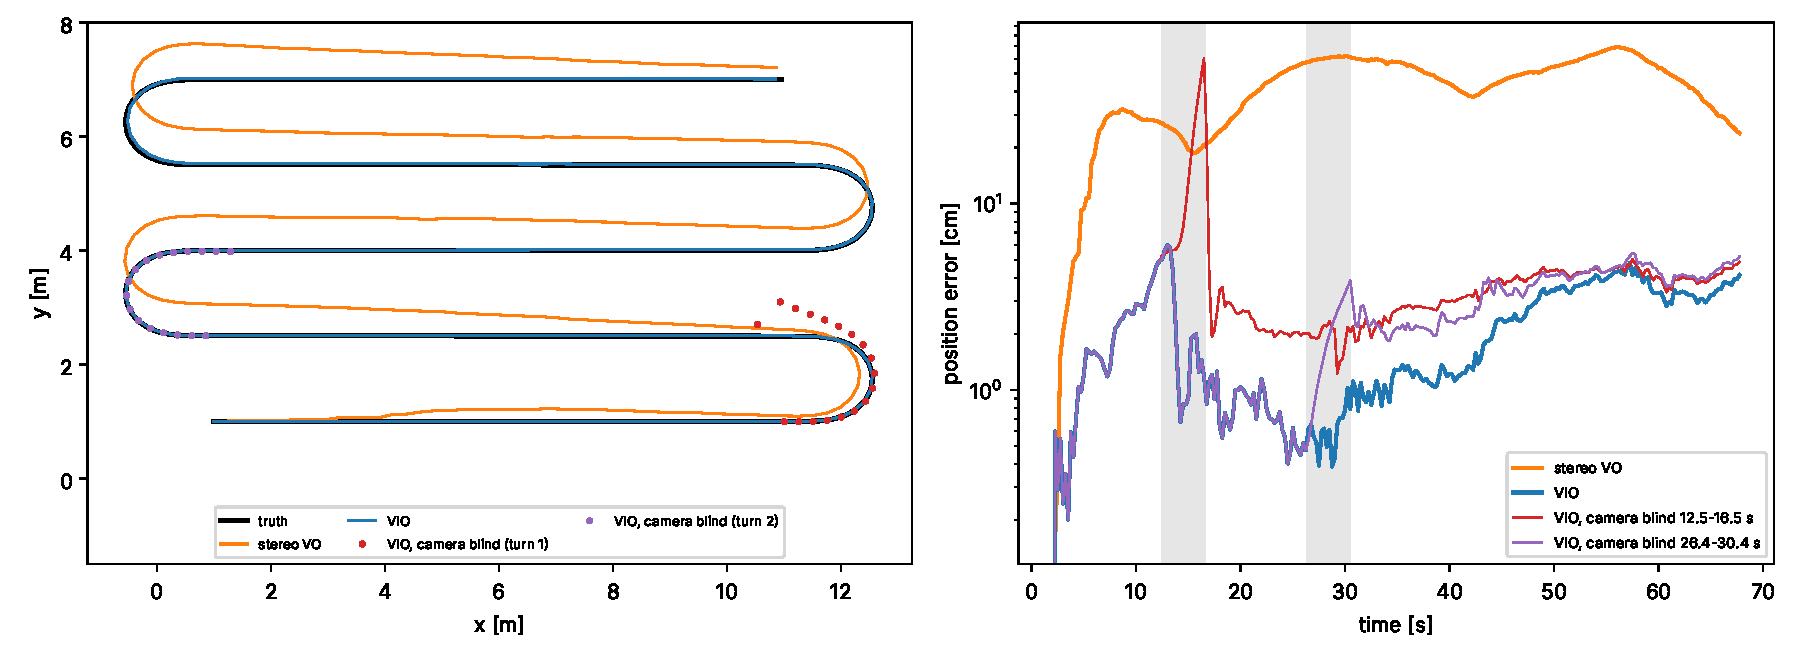
\includegraphics[width=\linewidth]{figures/ch13_traj.pdf}
\caption{The garden drive. Left: trajectories (red and purple dots: the
VIO while the camera is blind). Right: position errors. Stereo VO of
Chapter~\ref{ch:vo}: 46\,cm RMS. VIO: 2.5\,cm RMS. Camera blind for 4\,s
in the first turn: 60\,cm at the end of the blackout, before the
accelerometer bias is known; in the second turn: no visible effect.}
\label{fig:viotraj}
\end{figure}

The VIO reaches 2.5\,cm RMS and 4.1\,cm at the end, against 46\,cm RMS
for the stereo VO, with nothing but odometry: no loop closure. In
Python it processes the 68\,s in about 45\,s, faster than real time,
with some 670 landmarks and 1800 observations per window.

The two blackouts tell more. Blind for 4\,s during the \emph{second}
turn, the VIO coasts on the IMU and loses nothing: its error stays below
4\,cm. Blind during the \emph{first} turn, it drifts to 60\,cm. That is
$\frac12\cdot0.1\cdot4^2=0.8$\,m of accelerometer bias error, as
\cref{prop:drift} predicts: the bias was still unresolved, because the
row before was straight (\cref{prop:tiltbias}). Then, a second after the
camera comes back, the error falls back to 4\,cm. The returning images
fix the velocity, the turn fixes the bias, and the marginalisation prior,
which still remembers the IMU chain through the blackout and its
dependence on the bias, lets the smoother correct the blind stretch
retroactively.

\section{Calibration: extrinsics and time offset}

Two calibrations sit between the sensors. The extrinsic transformation
$T_{BC}$ is observable under rotation about two or more axes and is
best estimated offline with a calibration target (Kalibr) and then kept
fixed or refined online. The time offset $t_d$ between the two clocks
is subtler, and cheap to get wrong.

\begin{proposition}{A time offset is a motion error}{timeoffset}
If the image stamped $t$ is taken at $t+t_d$, it shows the camera pose
$T(t+t_d)\approx T(t)\Exp\bigl(t_d(\vect{v}^b,\bomega)\bigr)$, where
$\vect{v}^b$ and $\bomega$ are the body-frame linear and angular
velocities. To first order the estimator sees the pose displaced by
$t_d\vect{v}^b$ and rotated by $t_d\bomega$.
\end{proposition}

\begin{proof}
A first-order Taylor expansion of $s\mapsto T(t+s)$ in the right
trivialisation: $T(t)^{-1}\dot T(t)$ is the twist $(\vect{v}^b,\bomega)$
in the body frame (with the lever arm of the camera, which changes
$\vect{v}^b$ but not $\bomega$).
\end{proof}

At constant velocity the displacement $t_d\vect{v}^b$ is the same at
every keyframe and does little harm. In a turn at $\dot\psi=1.6$\,rad/s,
an offset of 10\,ms rotates the image by $0.9^\circ$ against the
gyroscope. The gyroscope's rotation is precise, so the optimiser
explains the shifted image of the scene ahead by a sideways
translation: \cref{prop:rtambig} with the scene at distance $d$ gives
about $t_d\dot\psi\,d\approx0.016\times10=16$\,cm per turn, and the
error stays after the turn.

\begin{figure}[ht]
\centering
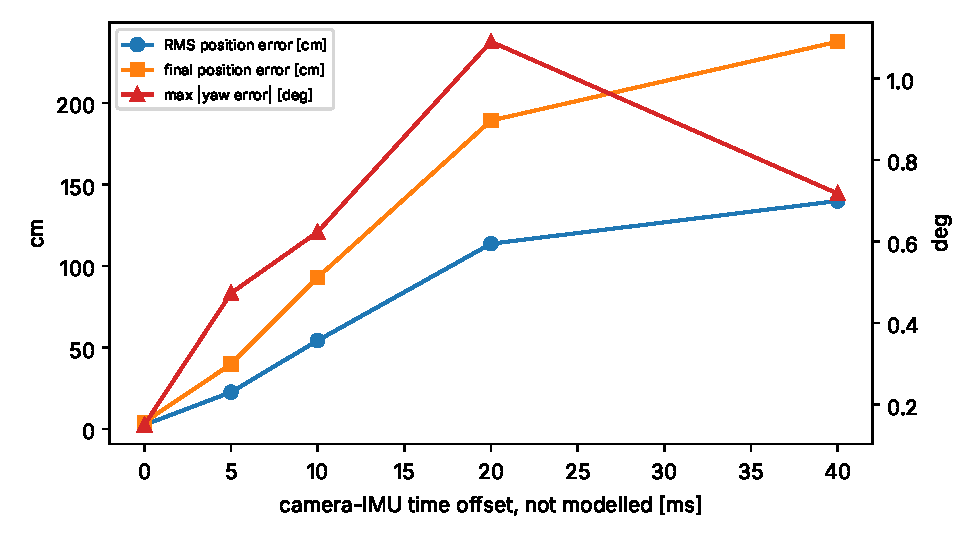
\includegraphics[width=0.62\linewidth]{figures/ch13_td.pdf}
\caption{Error of the VIO when the camera's timestamps are late by
$t_d$, not modelled. The error accumulates in the turns, sideways.}
\label{fig:viotd}
\end{figure}

\Cref{fig:viotd} confirms it: 5\,ms costs 40\,cm at the end of the drive
and 10\,ms costs 93\,cm, almost all of it accumulated in the four turns
and across the rows. The remedies are a shared clock (hardware
triggering, or a sensor that timestamps both) or estimating $t_d$
online. Qin and Shen do the latter by shifting each feature along its
image velocity, $\vect{z}(t+t_d)\approx\vect{z}(t)+t_d\dot{\vect{z}}$,
which adds one unknown and is observable as soon as the camera rotates.

\begin{mower}
VIO is the core of the mower's localisation: it runs between loop
closures, survives a few seconds of glare or a camera blocked by a
branch, and keeps roll and pitch, which matter for slopes. Three
practical consequences. Begin every session with a turn: the
accelerometer bias is not known until the mower has rotated, and
\cref{fig:viotraj} shows what an early blackout costs. Synchronise the
camera and the IMU in hardware: the turns at the end of the rows are
exactly where a few milliseconds hurt. And remember that the
accelerometer bias problem of straight rows, and the four unobservable
directions, are what wheel odometry and RTK-GNSS will fix in
Chapter~14. For monocular VIO on ground vehicles, Wu et~al.\ show that
straight driving at constant acceleration also loses the scale.
\end{mower}

\begin{practice}[\code{vslam/vio.py}, \code{vslam/sim.py}
  (\code{GardenMotion}), \code{examples/ch13\_vio.py},
  \code{notebooks/ch13\_vio.ipynb}]
\begin{center}
\begin{tabular}{@{}ll@{}}
\toprule
Code & Formula\\
\midrule
\code{vio.stereo\_residuals} & \cref{prop:viojac}\\
\code{vio.SlidingWindowVIO} & \cref{def:swvio}, \cref{lem:schur}\\
\code{vio.gauge\_directions} & \eqref{eq:vionull}\\
\code{vio.msckf\_project} & \cref{prop:msckf}\\
\code{vio.static\_init} & \cref{prop:staticinit}\\
\code{vio.gyro\_bias\_from\_rotations} & \cref{prop:align}\\
\code{vio.align\_gravity\_velocity} & \cref{prop:align}\\
\code{sim.GardenMotion} & smooth drive, exact IMU\\
\bottomrule
\end{tabular}
\end{center}
The tests check the visual Jacobians against finite differences, the
accuracy of a short drive and the positive semidefiniteness of the
marginalisation prior, that the four directions of \eqref{eq:vionull}
annihilate the window Hessian while roll does not, the equivalence of
\cref{prop:msckf} with the Schur complement, the static initialisation,
and the recovery of gravity, velocities and gyroscope bias by
alignment.
\end{practice}

\section*{Further reading and C++ pointers}
\addcontentsline{toc}{section}{Further reading and C++ pointers}

Filters: A.~I.~Mourikis and S.~I.~Roumeliotis (ICRA 2007), M.~Li and
A.~I.~Mourikis (IJRR 2013) on consistency, G.~Huang et~al.\ on
observability-constrained estimation, and OpenVINS (P.~Geneva et~al.,
ICRA 2020). Smoothers: OKVIS (S.~Leutenegger et~al., IJRR 2015),
VINS-Mono (T.~Qin, P.~Li and S.~Shen, IEEE T-RO 2018), and ORB-SLAM3
(C.~Campos et~al., IEEE T-RO 2021). Observability: E.~S.~Jones and
S.~Soatto (IJRR 2011), J.~Kelly and G.~S.~Sukhatme (IJRR 2011),
J.~A.~Hesch et~al.\ (IEEE T-RO 2014). Ground vehicles: K.~J.~Wu et~al.,
``VINS on wheels'' (ICRA 2017). Time offset: T.~Qin and S.~Shen (IROS
2018), M.~Li and A.~I.~Mourikis (IJRR 2014). Calibration: Kalibr
(P.~Furgale, J.~Rehder and R.~Siegwart, IROS 2013). In C++: OpenVINS,
VINS-Fusion, OKVIS2, Basalt, ORB-SLAM3, and GTSAM's
\code{CombinedImuFactor} with its incremental smoother.

\FloatBarrier
\section*{Exercises}
\addcontentsline{toc}{section}{Exercises}

\begin{enumerate}[label=\textbf{13.\arabic*},ref=13.\arabic*]
\item\label{ex:13null} Show that a rotation about a horizontal axis is
  not a symmetry of \eqref{eq:swcost}, unless the accelerometer biases
  change too, and compute how much they must change for a $1^\circ$ tilt.
\item\label{ex:13count} Count the degrees of freedom of a window of $N$
  keyframes, and the unknowns of the reduced system in our
  implementation. Why is eliminating the landmarks first the right
  order, and what would change if the landmarks were kept and the states
  eliminated?
\item\label{ex:13msckf} A feature is seen in $m=2$ camera poses. How
  many constraints on the poses does the MSCKF extract from it? And for
  a stereo feature (three measurements per pose)?
\item\label{ex:13td} Estimate the sideways error per turn caused by a
  time offset of 2\,ms, for a turn at $1.6$\,rad/s and a scene 10\,m
  away. What clock accuracy makes it negligible next to the VIO's
  2.5\,cm?
\end{enumerate}

\subsection*{Solutions}

\textbf{13.1.} By the proof of \cref{prop:tiltbias}, a rotation
$\Exp(\delta\btheta)$ about a horizontal axis changes the predicted specific
force by $R\T(\delta\btheta\times\vect{g})$, of norm $g|\delta\btheta|$, which
no residual absorbs unless the biases change by $-R\T(\delta\btheta\times
\vect{g})$; and if the body rotates in the window, no constant change
does. For $1^\circ$: $9.81\times0.01745=0.17$\,m/s$^2$.

\textbf{13.2.} $15N$ state unknowns plus $3L$ for $L$ landmarks: here
$120+3\times670\approx2130$. Eliminating the $L$ landmarks costs one
$3\times3$ inverse each, because their block of the Hessian is block
diagonal; the reduced system is $120\times120$ and dense. Eliminating
the states first would fill in the landmark block (every pair of
landmarks seen from a common keyframe would become coupled), leaving a
$2000\times2000$ dense system.

\textbf{13.3.} With $m=2$ monocular observations, $\vect{r}$ has 4 rows
and $H_f$ 3 columns, so $N$ has $4-3=1$ column: one constraint, the
epipolar constraint between the two poses. A stereo feature in two poses
gives $6-3=3$ constraints: the second stereo pair measures the point
again, so its full position relative to the first pose constrains the
relative pose.

\textbf{13.4.} $t_d\dot\psi\,d=0.002\times1.6\times10=3.2$\,cm per turn,
already more than the VIO's error. To bring it down to about 3\,mm per
turn, $t_d$ must be below about 0.2\,ms: in practice, hardware
synchronisation, or online estimation of $t_d$.
